\section{Evaluation}\label{sec:experiments}
\subsection{Setup}
\subsubsection{Environment}
Most of the experiments were performed on a single machine with two Intel Xeon Processor E5--2699 v4 CPUs, 64 GB of RAM,
and a 800GB SSD\@.
Memory caches were dropped before each experiment to force disk loads.
\subsubsection{Datasets and Queries}
We use real-world data graphs~\cite{snapnets} listed in Table~\ref{tab:datasets}.
The datasets come from difference domains of application, and they range in different size.
The vertices and edges in the datasets are labeled randomly as in~\cite{DBLP:journals/pvldb/MhedhbiS19}.

The queries (Figure~\ref{img:queries}) are selected and edited from existing work~\cite{DBLP:conf/cloud/SerafiniMS17,DBLP:journals/pvldb/MhedhbiS19}.
The labels of vertices and edges are tagged randomly,
and they are represented by the color and the style of lines in Figure~\ref{img:queries}.
The queries we choose represent different topologies: trees, chains, and cyclic graphs.
$q_9$ --- $q_{12}$ are queries with multi-edges.
\begin{table}
  \caption{Datasets}\label{tab:datasets}
  \begin{tabular}{lrrr}
    \toprule
    Name & $|V|$ & $|E|$ & \parbox[t][][t]{0.18\linewidth}{Time of Pre-processing (in sec)} \\
    \midrule
    soc-Epinions (EP) & 76K & 509K & 0.321 \\
    web-Google (GO) & 876K & 5.1M & 4.530 \\
    web-BerkStan (BS) & 685K & 7.6M & 5.240 \\
    soc-LiveJournal (LJ) & 4.8M & 69M & 55.095 \\
    com-Orkut (OK) & 3.1M & 117.2M & 100.323 \\
    \bottomrule
  \end{tabular}
\end{table}

\begin{figure}[ht]
  \centering
  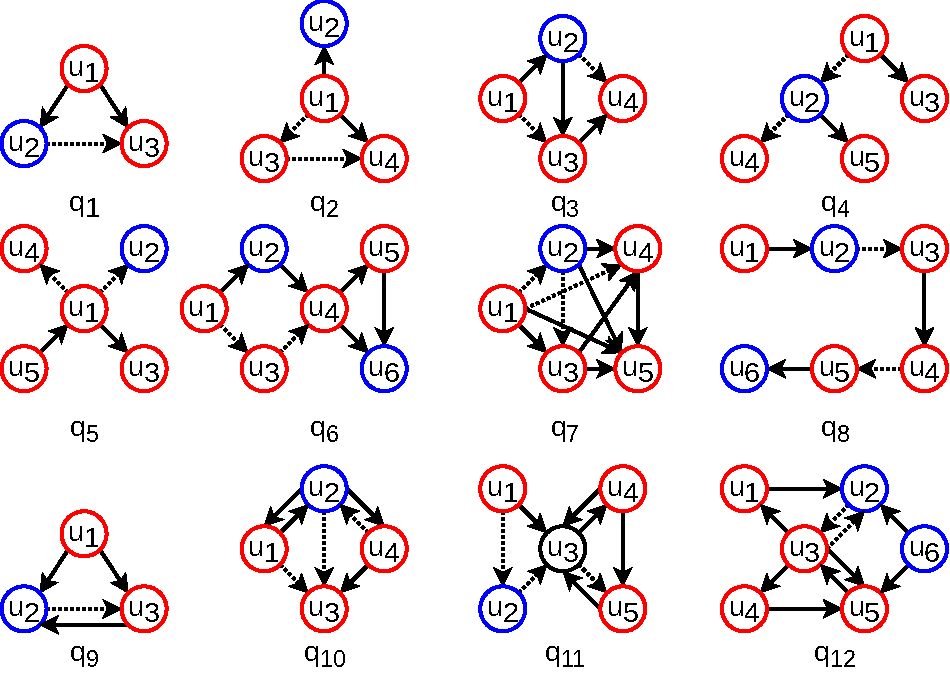
\includegraphics[width=0.5\textwidth]{img/queries.pdf}
  \caption{The queries.}\label{img:queries}
\end{figure}

\subsection{Pre-processing Cost}
\subsection{Comparative Performance}
\subsection{Compression Ratio}
\subsection{Performance of Star Decompression}
\subsection{Parallelism of Pipeline Join}
